\section{Anwendungen in der anorganischen Chemie}
\subsection{[SIMesPGa\textit{t}Bu$_2$]$_2$, [SIMesP(Ga\textit{t}Bu$_2$)$_2$Cl] und [K(SIMesP)$_3$Al\textit{t}Bu]}
\subsection{[Hg$_8$Te$_8$(Te$_2$)$_4$]$^{8-}$: Ein anorganisches Porphyrin?}
\begin{figure}[ht!]
	\centering
	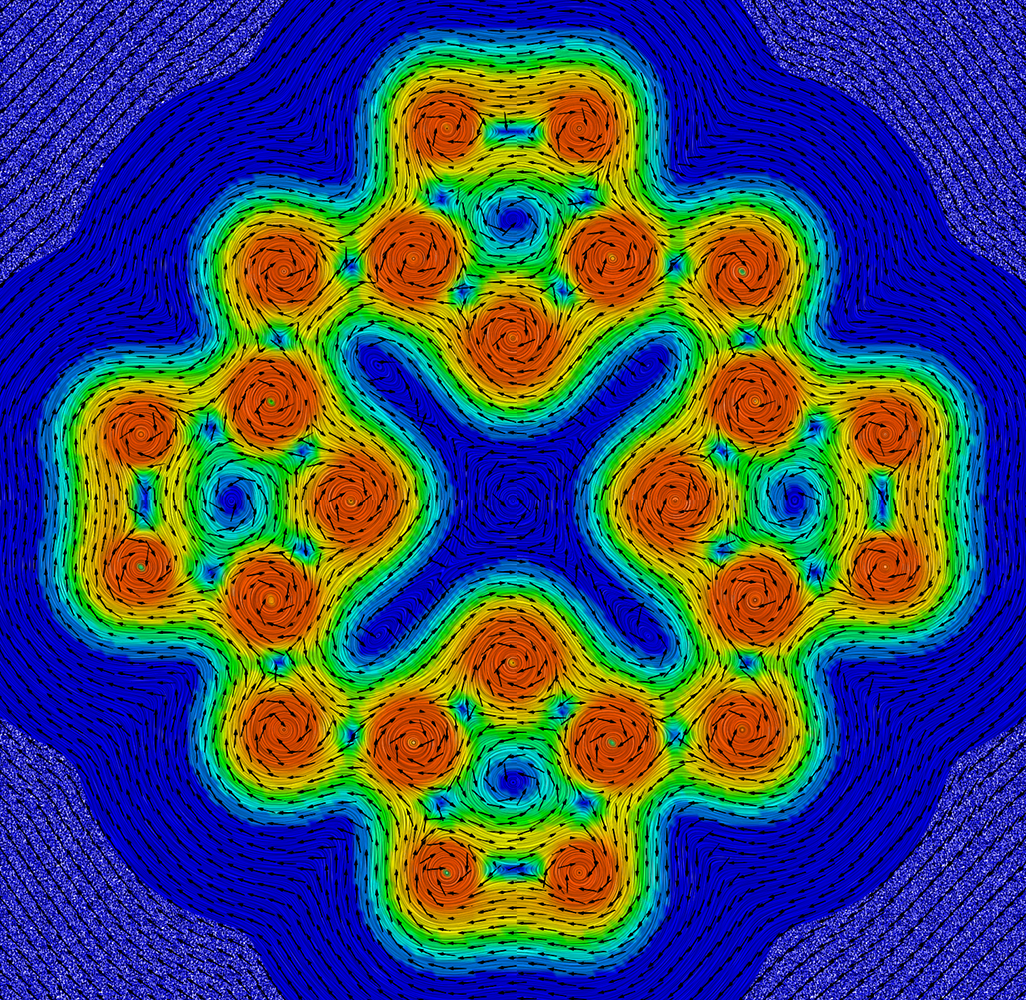
\includegraphics[width=0.6\textwidth]{hgte_1bohr}
	\captionsetup{figurewithin = chapter}
	\captionsetup{font=small, labelfont=bf}\caption[]{.}
\label{abb:hgtelic}
\end{figure}

\begin{figure}[ht!]
	\centering
	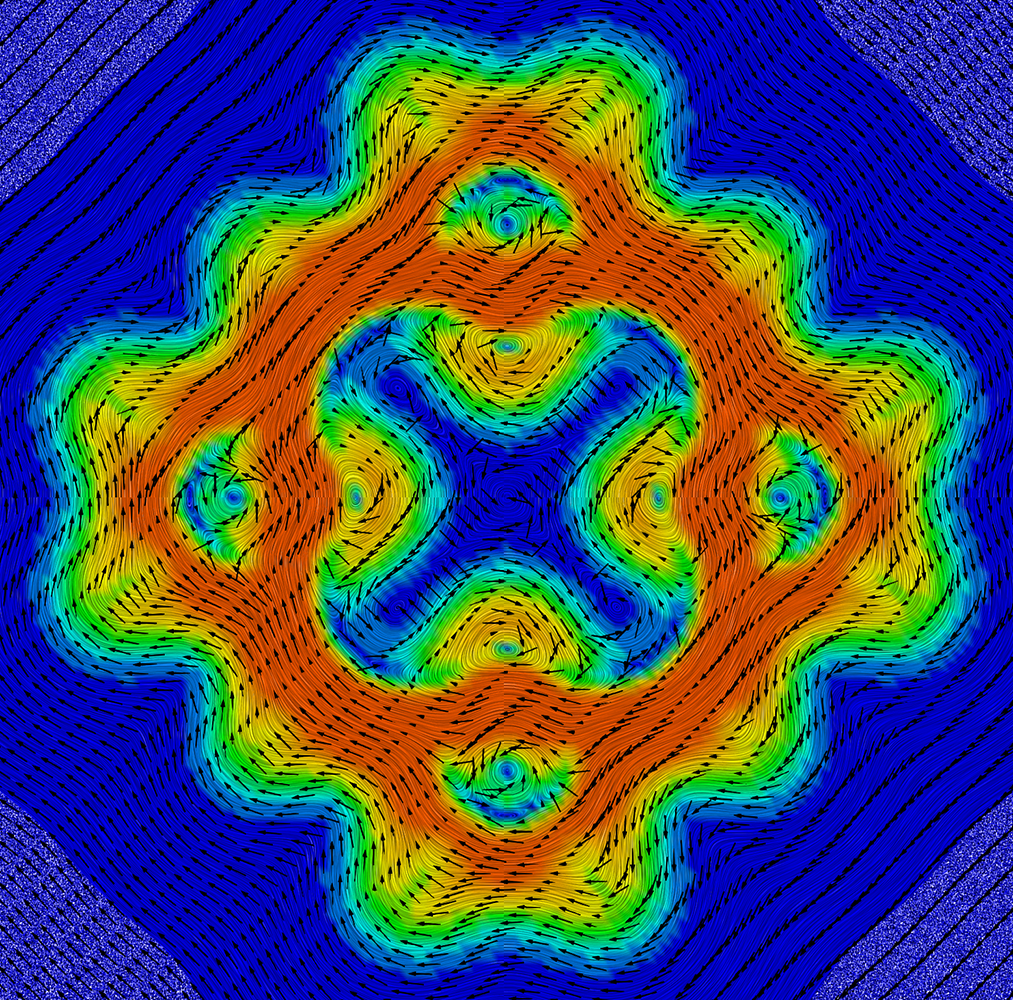
\includegraphics[width=0.6\textwidth]{porph_1bohr}
	\captionsetup{figurewithin = chapter}
	\captionsetup{font=small, labelfont=bf}\caption[]{.}
\label{abb:porphlic}
\end{figure}

\begin{figure}[ht!]
	\centering
	\includegraphics[width=0.6\textwidth]{b8s16_1bohr}
	\captionsetup{figurewithin = chapter}
	\captionsetup{font=small, labelfont=bf}\caption[]{.}
\label{abb:b8s16hlic}
\end{figure}

\begin{figure}[ht!]
	\centering
	\includegraphics[width=0.6\textwidth]{b8se16_1bohr}
	\captionsetup{figurewithin = chapter}
	\captionsetup{font=small, labelfont=bf}\caption[]{.}
\label{abb:b8se16hlic}
\end{figure}
\subsection{[Co\@Sn$_6$Sb$_6$]$^{3-}$}
\section{Ringströme in großen ringförmigen Kohlenstoffnanoröhren}